\documentclass[border=14pt]{standalone}
\usepackage[T1]{fontenc}
\usepackage[default]{sourcesanspro}
\usepackage{tikz}
\usepackage{xcolor}
\usetikzlibrary{arrows.meta}

\definecolor{LineBlue}{RGB}{65,105,225}
\definecolor{DotColor}{RGB}{34,120,34}
\definecolor{ErrRed}{RGB}{200,40,40}

% Coordinate convention
%   TikZ x = height - 155   (range 0..45, for h in 155..200 cm)
%   TikZ y = shoe   - 35    (range 0..12, for s in 35..47 EU)
%   Scale: x=0.22cm per unit, y=0.65cm per unit

\begin{document}
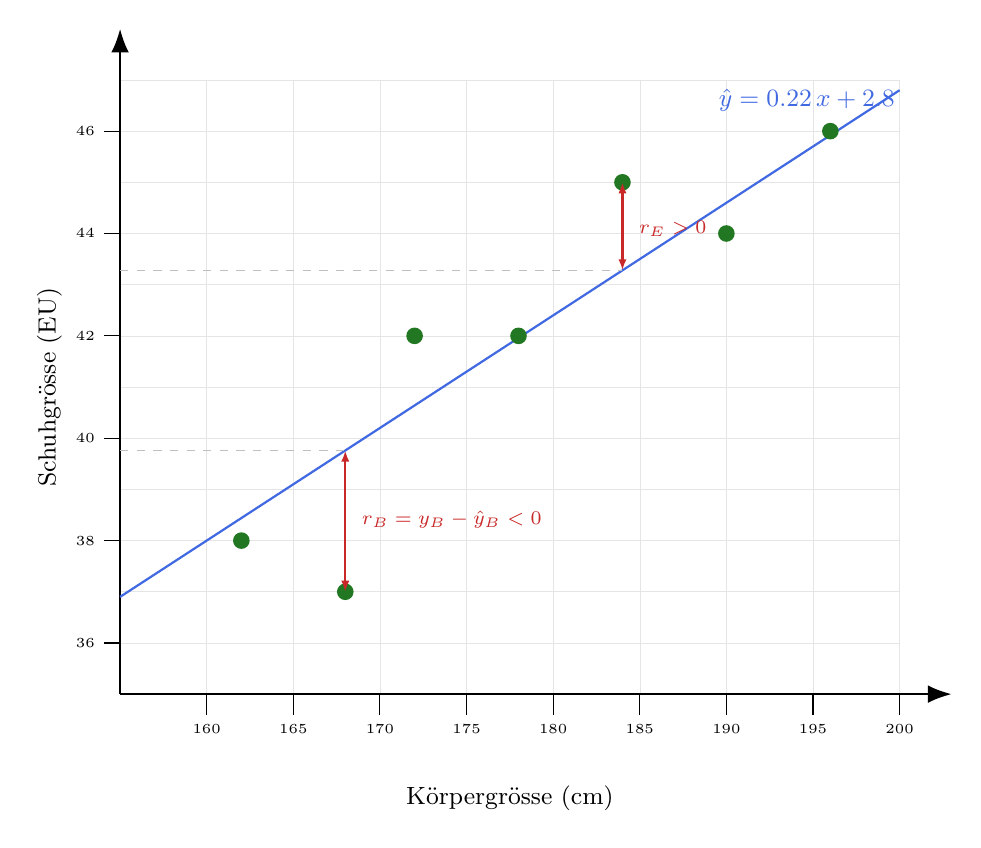
\begin{tikzpicture}[x=0.22cm, y=0.65cm]

  % --- Grid ---
  \draw[gray!20, very thin, xstep=5, ystep=1] (0,0) grid (45,12);

  % --- Axes ---
  \draw[thick,-{Latex[length=3mm]}] (0,0) -- (48,0);
  \draw[thick,-{Latex[length=3mm]}] (0,0) -- (0,13);

  % --- X ticks: h = 160,165,...,200 ---
  \foreach \h in {160,165,170,175,180,185,190,195,200} {
    \pgfmathsetmacro{\xtz}{\h - 155}
    \draw (\xtz, 0) -- (\xtz, -0.4) node[below, font=\tiny] {\h};
  }
  \node[font=\small, anchor=north] at (22.5, -1.6) {Körpergrösse (cm)};

  % --- Y ticks: s = 36,38,40,42,44,46 ---
  \foreach \s in {36,38,40,42,44,46} {
    \pgfmathsetmacro{\ytz}{\s - 35}
    \draw (0, \ytz) -- (-0.9, \ytz) node[left, font=\tiny] {\s};
  }
  \node[font=\small, rotate=90, anchor=south] at (-2.8, 6) {Schuhgrösse (EU)};

  % --- Regression line: ŷ = 0.22·h + 2.8 ---
  %   At h=155 (x=0):  ŷ = 36.9  → y_tz = 1.9
  %   At h=200 (x=45): ŷ = 46.8  → y_tz = 11.8
  \draw[LineBlue, thick] (0, 1.9) -- (45, 11.8);
  \node[LineBlue, font=\small, anchor=south west] at (34, 11.2)
      {$\hat{y} = 0.22\,x + 2.8$};

  % --- Data points (TikZ coords: (h-155, s-35)) ---
  %  A: h=162, s=38  → (7,  3)   near line
  %  B: h=168, s=37  → (13, 2)   BELOW line  ← residual illustrated
  %  C: h=172, s=42  → (17, 7)   above line
  %  D: h=178, s=42  → (23, 7)   near line
  %  E: h=184, s=45  → (29, 10)  ABOVE line  ← residual illustrated
  %  F: h=190, s=44  → (35, 9)   below line
  %  G: h=196, s=46  → (41, 11)  near line
  \fill[DotColor]
    ( 7,  3) circle (3pt)
    (13,  2) circle (3pt)
    (17,  7) circle (3pt)
    (23,  7) circle (3pt)
    (29, 10) circle (3pt)
    (35,  9) circle (3pt)
    (41, 11) circle (3pt)
    ;

  % --- Residual B: actual (13,2), line at x=13 → y = 1.9 + 0.22·13 = 4.76 ---
  %   Arrow from ŷ_B up to actual (negative residual, point is below line)
  \draw[gray!50, dashed, thin] (0, 4.76) -- (13, 4.76);
  \draw[ErrRed, thick, {Latex[length=4pt]}-{Latex[length=4pt]}] (13, 2) -- (13, 4.76);
  \node[ErrRed, font=\scriptsize, anchor=west] at (13.4, 3.4)
      {$r_B = y_B - \hat{y}_B < 0$};

  % --- Residual E: actual (29,10), line at x=29 → y = 1.9 + 0.22·29 = 8.28 ---
  %   Arrow from ŷ_E up to actual (positive residual, point is above line)
  \draw[gray!50, dashed, thin] (0, 8.28) -- (29, 8.28);
  \draw[ErrRed, thick, {Latex[length=4pt]}-{Latex[length=4pt]}] (29, 8.28) -- (29, 10);
  \node[ErrRed, font=\scriptsize, anchor=west] at (29.4, 9.1)
      {$r_E > 0$};

\end{tikzpicture}
\end{document}
